\documentclass{standalone}
\usepackage{tikz}
\usetikzlibrary{patterns}
\usetikzlibrary{positioning}
\usetikzlibrary{patterns, positioning}
\usetikzlibrary{shapes.misc}
\usepackage[outline]{contour}
\contourlength{1.5pt} 
\usepackage[sfdefault]{ClearSans}

\begin{document}
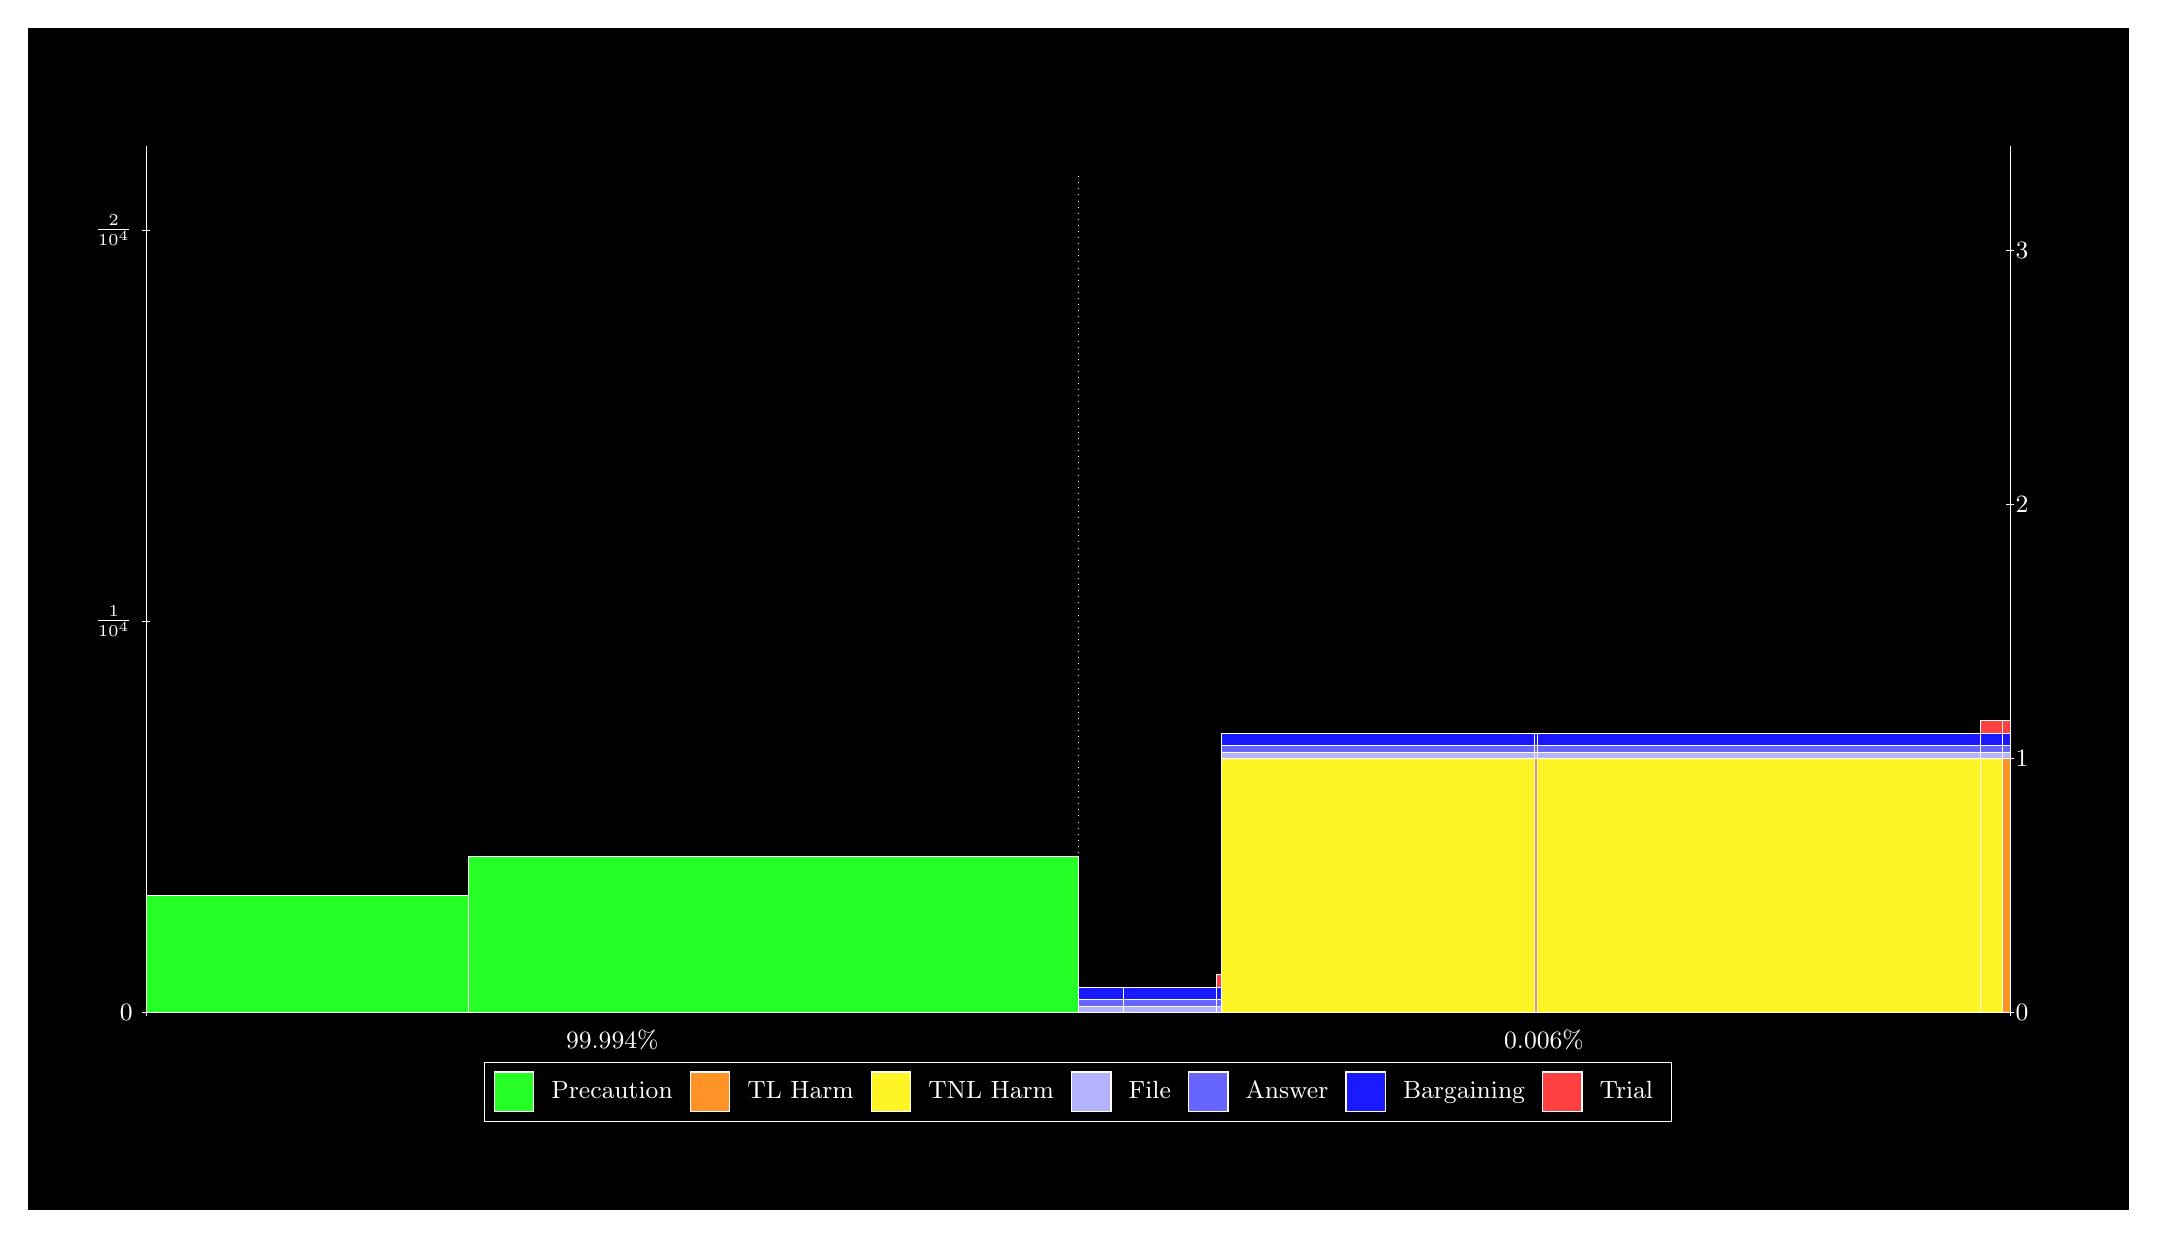
\begin{tikzpicture}
\draw[fill=black] (0,0) rectangle (26.667,15);
\draw[fill=green!85,draw=white,very thin] (1.5,2.5) rectangle (5.5948,3.9905);
\draw[fill=green!85,draw=white,very thin] (5.5948,2.5) rectangle (13.333,4.4874);
\draw[fill=green!85,draw=white,very thin] (13.333,2.5) rectangle (13.901,2.5001);
\draw[fill=blue!30,draw=white,very thin] (13.333,2.5001) rectangle (13.901,2.5808);
\draw[fill=blue!60,draw=white,very thin] (13.333,2.5808) rectangle (13.901,2.6614);
\draw[fill=blue!90,draw=white,very thin] (13.333,2.6614) rectangle (13.901,2.8228);
\draw[fill=green!85,draw=white,very thin] (13.901,2.5) rectangle (15.093,2.5001);
\draw[fill=blue!30,draw=white,very thin] (13.901,2.5001) rectangle (15.093,2.5808);
\draw[fill=blue!60,draw=white,very thin] (13.901,2.5808) rectangle (15.093,2.6615);
\draw[fill=blue!90,draw=white,very thin] (13.901,2.6615) rectangle (15.093,2.8228);
\draw[fill=green!85,draw=white,very thin] (15.093,2.5) rectangle (15.155,2.5001);
\draw[fill=blue!30,draw=white,very thin] (15.093,2.5001) rectangle (15.155,2.5808);
\draw[fill=blue!60,draw=white,very thin] (15.093,2.5808) rectangle (15.155,2.6614);
\draw[fill=blue!90,draw=white,very thin] (15.093,2.6614) rectangle (15.155,2.8228);
\draw[fill=red!75,draw=white,very thin] (15.093,2.8228) rectangle (15.155,2.9841);
\draw[fill=green!85,draw=white,very thin] (15.155,2.5) rectangle (19.122,2.5001);
\draw[fill=yellow!85,draw=white,very thin] (15.155,2.5001) rectangle (19.122,5.7269);
\draw[fill=blue!30,draw=white,very thin] (15.155,5.7269) rectangle (19.122,5.8076);
\draw[fill=blue!60,draw=white,very thin] (15.155,5.8076) rectangle (19.122,5.8883);
\draw[fill=blue!90,draw=white,very thin] (15.155,5.8883) rectangle (19.122,6.0496);
\draw[fill=green!85,draw=white,very thin] (19.122,2.5) rectangle (19.16,2.5001);
\draw[fill=orange!85,draw=white,very thin] (19.122,2.5001) rectangle (19.16,5.7269);
\draw[fill=blue!30,draw=white,very thin] (19.122,5.7269) rectangle (19.16,5.8076);
\draw[fill=blue!60,draw=white,very thin] (19.122,5.8076) rectangle (19.16,5.8883);
\draw[fill=blue!90,draw=white,very thin] (19.122,5.8883) rectangle (19.16,6.0496);
\draw[fill=green!85,draw=white,very thin] (19.16,2.5) rectangle (24.788,2.5001);
\draw[fill=yellow!85,draw=white,very thin] (19.16,2.5001) rectangle (24.788,5.727);
\draw[fill=blue!30,draw=white,very thin] (19.16,5.727) rectangle (24.788,5.8076);
\draw[fill=blue!60,draw=white,very thin] (19.16,5.8076) rectangle (24.788,5.8883);
\draw[fill=blue!90,draw=white,very thin] (19.16,5.8883) rectangle (24.788,6.0496);
\draw[fill=green!85,draw=white,very thin] (24.788,2.5) rectangle (25.072,2.5001);
\draw[fill=yellow!85,draw=white,very thin] (24.788,2.5001) rectangle (25.072,5.7269);
\draw[fill=blue!30,draw=white,very thin] (24.788,5.7269) rectangle (25.072,5.8076);
\draw[fill=blue!60,draw=white,very thin] (24.788,5.8076) rectangle (25.072,5.8883);
\draw[fill=blue!90,draw=white,very thin] (24.788,5.8883) rectangle (25.072,6.0496);
\draw[fill=red!75,draw=white,very thin] (24.788,6.0496) rectangle (25.072,6.2109);
\draw[fill=green!85,draw=white,very thin] (25.072,2.5) rectangle (25.167,2.5001);
\draw[fill=orange!85,draw=white,very thin] (25.072,2.5001) rectangle (25.167,5.7269);
\draw[fill=blue!30,draw=white,very thin] (25.072,5.7269) rectangle (25.167,5.8076);
\draw[fill=blue!60,draw=white,very thin] (25.072,5.8076) rectangle (25.167,5.8883);
\draw[fill=blue!90,draw=white,very thin] (25.072,5.8883) rectangle (25.167,6.0496);
\draw[fill=red!75,draw=white,very thin] (25.072,6.0496) rectangle (25.167,6.2109);
\draw[white,very thin] (1.5,2.5) -- (1.5,13.5);
\draw[white,very thin] (1.45,2.5) -- (1.55,2.5);
\node[font=\small,text=white, anchor=east] at (1.45, 2.5) {0};
\draw[white,very thin] (1.45,7.4685) -- (1.55,7.4685);
\node[font=\small,text=white, anchor=east] at (1.45, 7.4685) {$\frac{1}{10^{4}}$};
\draw[white,very thin] (1.45,12.437) -- (1.55,12.437);
\node[font=\small,text=white, anchor=east] at (1.45, 12.437) {$\frac{2}{10^{4}}$};

\draw[white,dotted,very thin] (13.333,2.83) -- (13.333,13.17);
\draw[white,very thin] (25.167,2.5) -- (25.167,13.5);
\draw[white,very thin] (25.117,2.5) -- (25.217,2.5);
\node[font=\small,text=white, anchor=west] at (25.117, 2.5) {0};
\draw[white,very thin] (25.117,5.7268) -- (25.217,5.7268);
\node[font=\small,text=white, anchor=west] at (25.117, 5.7268) {1};
\draw[white,very thin] (25.117,8.9537) -- (25.217,8.9537);
\node[font=\small,text=white, anchor=west] at (25.117, 8.9537) {2};
\draw[white,very thin] (25.117,12.18) -- (25.217,12.18);
\node[font=\small,text=white, anchor=west] at (25.117, 12.18) {3};

\draw[white,very thin] (1.5,2.5) -- (25.167,2.5);
\draw[white,very thin] (1.5,2.45) -- (1.5,2.55);
\node[font=\small,text=white, anchor=north] at (1.5, 2.45) {};
\draw[white,very thin] (25.167,2.45) -- (25.167,2.55);
\node[font=\small,text=white, anchor=north] at (25.167, 2.45) {};

\node[font=\small,text=white,anchor=south] at (7.4167, 1.9) {99.994\%};
\node[font=\small,text=white,anchor=south] at (19.25, 1.9) {0.006\%};
\draw (13.3333,2.5) node (B) {};
\begin{scope}[align=center]
\matrix[scale=0.5,draw=white,below=0.5cm of B,nodes={draw},column sep=0.1cm]{
\node[rectangle,draw,minimum width=0.5cm,minimum height=0.5cm,fill=green!85]{}; & \node[draw=none,font=\small,text=white]{Precaution}; &
\node[rectangle,draw,minimum width=0.5cm,minimum height=0.5cm,fill=orange!85]{}; & \node[draw=none,font=\small,text=white]{TL Harm}; &
\node[rectangle,draw,minimum width=0.5cm,minimum height=0.5cm,fill=yellow!85]{}; & \node[draw=none,font=\small,text=white]{TNL Harm}; &
\node[rectangle,draw,minimum width=0.5cm,minimum height=0.5cm,fill=blue!30]{}; & \node[draw=none,font=\small,text=white]{File}; &
\node[rectangle,draw,minimum width=0.5cm,minimum height=0.5cm,fill=blue!60]{}; & \node[draw=none,font=\small,text=white]{Answer}; &
\node[rectangle,draw,minimum width=0.5cm,minimum height=0.5cm,fill=blue!90]{}; & \node[draw=none,font=\small,text=white]{Bargaining}; &
\node[rectangle,draw,minimum width=0.5cm,minimum height=0.5cm,fill=red!75]{}; & \node[draw=none,font=\small,text=white]{Trial}; \\\\
};\end{scope}

\end{tikzpicture}
\end{document}